\documentclass[12pt,a4paper]{article}
\usepackage{rmpackages}																% usual packages
\usepackage{rmtemplate}																% graphic charter
\usepackage{rmexocptce}																% for DS with cptce eval

%\cfoot{} 													% if no page number is needed
%\renewcommand\arraystretch{1.5}		% stretch table line height

\begin{document}

\begin{header}
Chapitre 1 -- Corps purs et mélanges
\end{header}

\section{Rappels}

Correction du QCM rappels de collège : 1-c ; 2-a,c,f ; 3-b,d ; 4-a,d ; 5-a ; 6-b,d,e,f.

\begin{conseil}
Pour la dernière question, il est nécessaire de manipuler la formule de la masse volumique donnée à la question précédente.
Pour cela, on pourra utiliser plusieurs méthodes : méthode du \og triangle \fg{}, substitution par des chiffres, etc.
Ces outils sont rappelés dans la fiche \og Outils mathématiques\fg{}.
L'essentiel est de \textbf{trouver une méthode qui vous convient} et avec laquelle vous êtes à l'aise.
\end{conseil}

\begin{remarque}
\unit{1}{\meter^3} c'est grand !
Nous reviendrons sur les conversions au fur et à mesure.
Pour l'instant, il faut se rappeler de la signification des différents préfixes utilisés devant les unités : voir encore la fiche \og Outils mathématiques\fg{}.
\end{remarque}


\section{Corps purs et mélanges}
\label{sec:corps_purs_melanges}

\subsection{Corps pur ou mélange ?}

\begin{conseil}
Faire la première section de l'activité 1 : Corps pur ou mélange ?
\end{conseil}

\begin{exemple}
\emph{Voir la première section de l'activité 1 : Corps pur ou mélange ?}
\center
\begin{tabular}{c|c}
\textbf{Corps pur} & \textbf{Mélange} \\
\hline
Eau distillée & Médicament \\
Lingot d'or   & Sirop \\
Sel           & Peinture \\
Aluminium     & Moutarde \\
Sucre         & Air
\end{tabular}
\end{exemple}

\begin{definition}
Un \textbf{corps pur} est composé d'une seule espèce chimique.
\end{definition}


\begin{definition}
Un \textbf{mélange} est composé de plusieurs espèces chimiques.
\end{definition}

\begin{definition}
Une \textbf{espèce chimique} est un ensemble d'entités chimiques (atomes, ions, molécules, etc.) \textbf{identiques}.
Elle est représentée par un symbole chimique.
\end{definition}

\begin{remarque}
Les espèces chimiques atomiques sont celles dont le symbole figure dans le tableau périodique des éléments, ou table de Mendeleiev : \href{https://fr.wikipedia.org/wiki/Tableau_p\%C3\%A9riodique_des_\%C3\%A9l\%C3\%A9ments#/media/Fichier:Tableau_p\%C3\%A9riodique_des_\%C3\%A9l\%C3\%A9ments.svg}{tableau périodique}.
Les molécules sont obtenues en liant certains de ces atomes et les ions sont des espèces chargées positivement ou négativement, dérivées de ces atomes ou molécules.
\end{remarque}

\subsection{Mélange homogène ou hétérogène ?}

\begin{conseil}
Faire la deuxième section de l'activité 1 : Mélange homogène ou hétérogène ?
La partie \textbf{justification} est toute aussi importante que le classement des différentes substances.
Par exemple, l'eau de mer est un mélange homogène si l'on considère qu'il s'agit d'un mélange d'eau et de sel.
Mais si l'on considère que c'est un mélange d'eau, de sel, de sable, algues, etc., c'est un mélange hétérogène.
\end{conseil}

\begin{exemple}
\emph{Voir la deuxième section de l'activité 1 : Mélange homogène ou hétérogène ?}
\center
\begin{tabular}{c|c}
\textbf{Mélange homogène} & \textbf{Mélange hétérogène} \\
\hline
Lait                & Lait vu au microscope \\
Bronze              & Eau gazeuse \\
Eau de mer          & Vinaigrette \\
Jus filtré de pomme & Nuages \\
Thé infusé          & Granit \\
Air                 & Jus d'oranges pressées
\end{tabular}
\end{exemple}

\begin{remarque}
Après agitation, les constituants d'un mélange homogène sont indiscernables à l'œil nu.
Dans un mélange hétérogène, on distingue au moins deux constituants à l'œil nu même après agitation.
\end{remarque}

\begin{definition}
Deux liquides \textbf{miscibles} forment un mélange homogène.
Deux liquides \textbf{non-miscibles} forment un mélange hétérogène.
\end{definition}

\begin{remarque}
La notion de mélange homogène ou hétérogène n'est valable qu'à une échelle donnée : le lait est considéré comme un mélange homogène s'il est observé à l'œil nu, mais c'est un mélange hétérogène s'il est vu au microscope.
Il s'agit en réalité d'une émulsion d'eau et de graisses : on retrouve de très fines gouttelettes de graisses en suspension dans de l'eau.
C'est pour cette raison que le lait parait blanc.
\end{remarque}

\subsection{Représentation microscopique}

\begin{multicols}{3}
\center
\begin{tikzpicture}[scale=0.5]
\draw[line width = 2pt] (0,5) -- (0,0) -- (4,0) -- (4,5);
\draw[line width = 1.5pt, color=bleu_f] (0.5,0.5) circle (.4);
\draw[line width = 1.5pt, color=bleu_f] (1.5,0.7) circle (.4);
\draw[line width = 1.5pt, color=bleu_f] (2.6,0.5) circle (.4);
\draw[line width = 1.5pt, color=bleu_f] (3.5,1) circle (.4);
\draw[line width = 1.5pt, color=bleu_f] (2.4,1.5) circle (.4);
\draw[line width = 1.5pt, color=bleu_f] (3.4,1.9) circle (.4);
\draw[line width = 1.5pt, color=bleu_f] (0.6,1.4) circle (.4);
\draw[line width = 1.5pt, color=bleu_f] (1.5,1.7) circle (.4);
\draw[line width = 1.5pt, color=bleu_f] (0.6,2.4) circle (.4);
\draw[line width = 1.5pt, color=bleu_f] (2.1,2.4) circle (.4);
\draw[line width = 1.5pt, color=bleu_f] (3.0,2.7) circle (.4);
\draw[line width = 1.5pt, color=bleu_f] (1.4,3.0) circle (.4);
\draw[line width = 1.5pt, color=bleu_f] (2.3,3.3) circle (.4);
\draw[line width = 1.5pt, color=bleu_f] (3.5,3.4) circle (.4);
\draw[line width = 1.5pt, color=bleu_f] (0.5,3.3) circle (.4);
\end{tikzpicture}

Corps pur

(ex : eau pure)

\begin{tikzpicture}[scale=0.5]
\draw[line width = 2pt] (0,5) -- (0,0) -- (4,0) -- (4,5);
\draw[line width = 1.5pt, color=bleu_f] (0.5,0.5) circle (.4);
\draw[line width = 1.5pt, color=green_f] (1.5,0.7) circle (.4);
\draw[line width = 1.5pt, color=bleu_f] (2.6,0.5) circle (.4);
\draw[line width = 1.5pt, color=green_f] (3.5,1) circle (.4);
\draw[line width = 1.5pt, color=green_f] (2.4,1.5) circle (.4);
\draw[line width = 1.5pt, color=bleu_f] (3.4,1.9) circle (.4);
\draw[line width = 1.5pt, color=green_f] (0.6,1.4) circle (.4);
\draw[line width = 1.5pt, color=bleu_f] (1.5,1.7) circle (.4);
\draw[line width = 1.5pt, color=bleu_f] (0.6,2.4) circle (.4);
\draw[line width = 1.5pt, color=bleu_f] (2.1,2.4) circle (.4);
\draw[line width = 1.5pt, color=green_f] (3.0,2.7) circle (.4);
\draw[line width = 1.5pt, color=bleu_f] (1.4,3.0) circle (.4);
\draw[line width = 1.5pt, color=bleu_f] (2.3,3.3) circle (.4);
\draw[line width = 1.5pt, color=green_f] (3.5,3.4) circle (.4);
\draw[line width = 1.5pt, color=green_f] (0.5,3.3) circle (.4);
\end{tikzpicture}

Mélange homogène

(ex : eau + sirop)

\begin{tikzpicture}[scale=0.5]
\draw[line width = 2pt] (0,5) -- (0,0) -- (4,0) -- (4,5);
\draw[line width = 2pt] (0,5) -- (0,0) -- (4,0) -- (4,5);
\draw[line width = 1.5pt, color=bleu_f] (0.5,0.5) circle (.4);
\draw[line width = 1.5pt, color=bleu_f] (1.5,0.7) circle (.4);
\draw[line width = 1.5pt, color=bleu_f] (2.6,0.5) circle (.4);
\draw[line width = 1.5pt, color=bleu_f] (3.5,1) circle (.4);
\draw[line width = 1.5pt, color=bleu_f] (2.4,1.5) circle (.4);
\draw[line width = 1.5pt, color=bleu_f] (3.4,1.9) circle (.4);
\draw[line width = 1.5pt, color=bleu_f] (0.6,1.4) circle (.4);
\draw[line width = 1.5pt, color=bleu_f] (1.5,1.7) circle (.4);
\draw[line width = 1.5pt, color=orange_f] (0.6,2.4) circle (.4);
\draw[line width = 1.5pt, color=orange_f] (2.1,2.4) circle (.4);
\draw[line width = 1.5pt, color=orange_f] (3.0,2.7) circle (.4);
\draw[line width = 1.5pt, color=orange_f] (1.4,3.0) circle (.4);
\draw[line width = 1.5pt, color=orange_f] (2.3,3.3) circle (.4);
\draw[line width = 1.5pt, color=orange_f] (3.5,3.4) circle (.4);
\draw[line width = 1.5pt, color=orange_f] (0.5,3.3) circle (.4);
\end{tikzpicture}

Mélange hétérogène

(ex : eau + huile)
\end{multicols}

\section{Identification d'espèces chimiques}

\subsection{Tests caractéristiques chimiques}

\begin{itemize}
\item[•] Test d'identification de l'eau : \href{https://tinyurl.com/thbmmcd}{https://tinyurl.com/thbmmcd} : en présence d'eau, le sulfate de cuivre devient bleu.
\item[•] Test d'identification du dioxygène : \href{https://tinyurl.com/y4y7elaf}{https://tinyurl.com/y4y7elaf} : en présence de dioxygène, un buchette incandescente se rallume.
\item[•] Test d'identification du dihydrogène : \href{https://tinyurl.com/y6a4kqw6}{https://tinyurl.com/y6a4kqw6} : quand on approche une flamme du dihydrogène, une détonation se produit.
\item[•] Test d'identification du dioxyde de carbone : \href{https://tinyurl.com/lef4pb5}{https://tinyurl.com/lef4pb5} : en présence de dioxyde de carbone, l'eau de chaux se trouble.

\end{itemize}

\begin{conseil}
Utiliser les vidéos et/ou le livre page 19 pour légender les schémas de l'activité 2.
Pour le test caractéristique de l'eau, faire le schéma en respectant le schéma narratif en trois étapes : situation initiale, transition (flèche) et situation finale.
\end{conseil}

\subsection{Propriétés physiques}

Les corps purs ont des propriétés physiques qui permettent de les identifier, comme la masse volumique ou les températures de changement d'état.

\paragraph{\textcolor{black}{Masse volumique}}

\begin{definition}
La \textbf{masse volumique} $\rho$ d'une substance de masse $m$ et de volume $V$ s'exprime par :
\begin{equation}
\rho = \frac{m}{V}.
\nonumber
\end{equation}
\end{definition}

\begin{remarque}
Il faut faire attention aux unités : si la masse est exprimée en kilogrammes et le volume en litres par exemple, la masse volumique sera en kilogrammes par litre kg/L.
\end{remarque}

\begin{definition}
La \textbf{densité} $d$ d'un solide ou d'un liquide de masse volumique $\rho$ est définie par rapport à l'eau :
\begin{equation}
d = \frac{\rho}{\rho_\mathrm{eau}}.
\nonumber
\end{equation}
\end{definition}

\begin{remarque}
Pour calculer la densité, il faut que les masses volumiques soient exprimées dans la même unité !
\end{remarque}

\begin{conseil}
Faire les questions 2, 3 et 4 de l'activité 2
\end{conseil}

\paragraph{\textcolor{black}{Température de changement d'état}}

\begin{conseil}
Faire les questions 5 et 6 de l'activité 2.
\end{conseil}

\begin{conseil}
Regarder la vidéo \href{https://tinyurl.com/yxmtwo32}{https://tinyurl.com/yxmtwo32}.
\end{conseil}

\begin{figure}[h]
\center
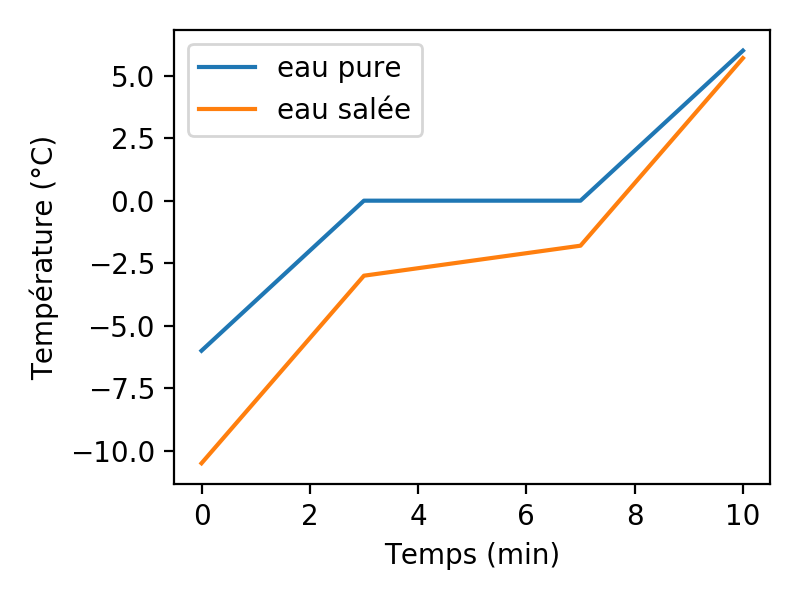
\includegraphics[scale=0.75]{../images/fusion.png}
\caption{Suivis thermométriques de la fonte de glace d'eau pure et de glace d'eau salée.}
\end{figure}

\begin{remarque}
Les courbes de suivi thermométrique sont les courbes que l'ont obtiendrait si l'on mesurait la température de l'eau du saladier de la vidéo régulièrement.
La première portion de droite correspond au chauffage des glaçons, la deuxième à la fonte et la troisième au chauffage de l'eau liquide.
\end{remarque}

\begin{definition}
Un corps pur \textbf{change d'état à température constante}.
Ce n'est pas le cas pour un mélange.
\end{definition}

\begin{conseil}
Faire la question 7 de l'activité 2.
\end{conseil}

\subsection{Chromatographie}

\begin{conseil}
Regarder la vidéo \href{https://tinyurl.com/y6neowtg}{https://tinyurl.com/y6neowtg}.
\end{conseil}

\begin{definition}
La chromatographie sur couche mince (CCM) permet de \textbf{séparer} et \textbf{identifier} les espèces chimiques présentes dans un mélange.
\end{definition}
Rq : pour un éluant et un support donnés, une espèce chimique migre de la même façon qu'elle soit pure ou présente dans un mélange.

\begin{figure}[h]
\center
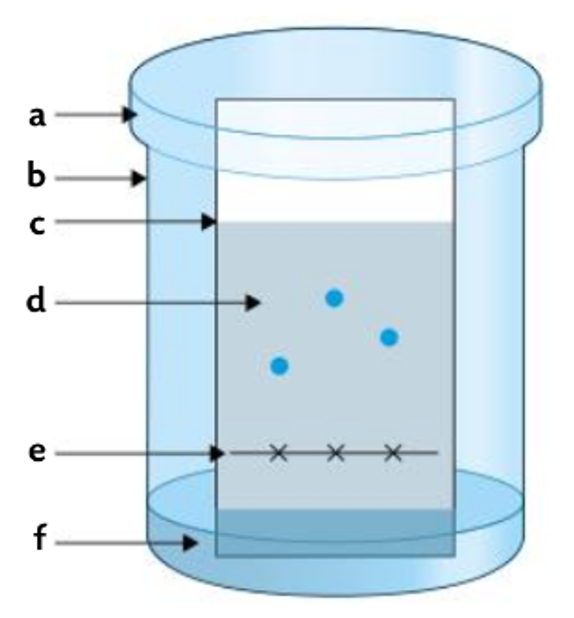
\includegraphics[scale=0.5]{../images/ccm_schema.png}
\caption{Schéma du montage expérimental utilisé pour réaliser une CCM.
a : coupelle, b : cuve, c : front de l'éluant, d : phase stationnaire, e : ligne de dépôt et f : phase mobile (éluant).}
\end{figure}

\begin{remarque}
Le schéma du montage expérimental n'est pas à connaitre mais il peut être bon de se familiariser avec le vocabulaire.
\end{remarque}

\section{Composition d'un mélange}

\begin{definition}
La \textbf{proportion en volume} d'une espèce E dans un mélange s'exprime comme le quotient du volume de cette espèce $V_\mathrm{E}$ par le volume total du mélange $V_\mathrm{tot}$ :
\begin{equation}
\frac{V_\mathrm{E}}{V_\mathrm{tot}}.
\nonumber
\end{equation}
Si elle est exprimée en pourcent, on parle de \textbf{pourcentage volumique}.
\end{definition}

\begin{remarque}
Pour calculer la proportion en volume, il faut que les deux volumes aient la même unité !
La proportion en volume (le pourcentage volumique) d'une espèce dans un mélange ne peut être supérieur à 1 (à \unit{100}{\%}) !
\end{remarque}

\begin{conseil}
Faire l'activité 3.
\end{conseil}

\begin{definition}
Le pourcentage volumique de diazote dans l'air est \unit{78}{\%}.
Le pourcentage volumique de dioxygène dans l'air est \unit{21}{\%}.
La masse volumique de l'air est d'environ \unit{1}{\gram/L}.
\end{definition}

\end{document}